% ============================================================
% Collateral Damage in Graph-based Memory Forgetting:
% Quantification, Exploitation, and Defense
% SCALE Workshop @ ICML 2026 (7-page version)
% ============================================================
\documentclass{article}

\usepackage{microtype}
\usepackage{graphicx}
\usepackage{subcaption}
\usepackage{booktabs}
\usepackage{hyperref}

\newcommand{\theHalgorithm}{\arabic{algorithm}}

% Blind review version
\usepackage{icml2026}

\usepackage{amsmath,amssymb}
\usepackage[capitalize,noabbrev]{cleveref}
\usepackage{multirow}
\usepackage{algorithm}
\usepackage{algorithmic}
\usepackage{xcolor}

% --- Custom Commands ---
\newcommand{\attraware}{\textsc{Attr-Aware}}
\newcommand{\bfsprop}{\textsc{BFS}}
\newcommand{\finding}[1]{\vspace{2pt}\noindent\textbf{Finding #1.}~}

\icmltitlerunning{Collateral Damage in Graph-based Memory Forgetting}

\begin{document}

\twocolumn[
  \icmltitle{Collateral Damage in Graph-based Memory Forgetting:\\
  Quantification, Exploitation, and Defense}

  \icmlaffiliation{anon}{Anonymous Institution}

  \begin{icmlauthorlist}
    \icmlauthor{Anonymous}{anon}
  \end{icmlauthorlist}

  \icmlcorrespondingauthor{Anonymous}{anonymous@example.com}

  \icmlkeywords{AI Agent Memory, Graph Propagation, Selective Forgetting, Adversarial Attacks}

  \vskip 0.3in
]

\printAffiliationsAndNotice{}

% ============================================================
\begin{abstract}
Agent memory systems increasingly use entity graphs for retrieval and consolidation, but invalidation is handled at the level of individual facts---leaving dependent facts silently stale.
Propagating invalidation through graph edges is a natural way to maintain consistency, yet \textbf{structural co-occurrence does not imply dependency}.
We study this design choice by implementing BFS invalidation propagation over co-occurrence graphs derived from MemoryAgentBench.
Across 6K--64K turns, BFS propagation reduces stale retention but damages 69--79\% of valid memories. It also degrades cross-task retrieval F1 by $10.1$pp.
Hub-targeted invalidations amplify this failure: five injected facts degrade 57.3\% of valid memories under white-box access.
To mitigate over-propagation, we propose \textbf{\attraware{} Selective Propagation}, an attribute-keyed directional filter that limits cascades to plausible dependency paths. It requires no LLM calls during propagation and achieves 78--100\% defense effectiveness.
Our results suggest that graph-based memory forgetting should incorporate dependency-aware propagation rather than raw co-occurrence traversal.
\end{abstract}

% ============================================================
\section{Introduction}
\label{sec:intro}

AI agents with persistent memory are moving from prototypes to production.
Mem0~\citep{mem0_2024} and other memory-augmented agent frameworks have proliferated across open-source and proprietary ecosystems~\citep{graph_agent_memory_survey_2026}.
These systems increasingly maintain entity graphs to organize stored facts~\citep{mem0_2024, magma_2026, zep_2025}, and emerging multimodal agent architectures face the same challenge of maintaining consistency across modalities that share entity references.

As memory scales to tens of thousands of facts, maintaining consistency becomes critical---yet multi-hop conflict resolution accuracy remains below 6\% on standard benchmarks~\citep{memoryagentbench_2026}.
The gap is structural: current systems handle invalidation \textit{individually}, leaving dependent facts silently stale.
Graph-based propagation---cascading updates through entity connections---is a plausible extension.
Zep~\citep{zep_2025} maintains temporal validity windows on graph edges; MAGMA~\citep{magma_2026} constructs explicit causal sub-graphs; Mem0~\citep{mem0_2024} operates conflict detection over a traversable entity graph.
Each implements prerequisites for propagation without taking the final step.

We implement this step and reveal a fundamental tension.
Entity co-occurrence graphs link facts that share entities, but sharing an entity does not imply causal dependency.
``The president of Russia'' connects diplomatic facts and unrelated economic facts identically.
Co-occurrence is not an artifact of naive graph construction: even typed-relation graphs contain co-occurrence as an unavoidable substructure whenever multiple facts reference the same entity.
BFS propagation treats all such connections identically, cascading invalidation through semantically meaningless edges.

This distinction---well-understood in transportation network resilience, where directional failure models separate correlated from causally dependent links~\citep{chen_network_2007}---has not been applied to AI memory systems.
We contribute:

\begin{enumerate}
  \item \textbf{Failure formulation}: We formalize invalidation propagation as a \textit{retention-forgetting trade-off} in graph-based agent memory: insufficient propagation leaves stale facts, while raw co-occurrence propagation damages valid memories (\cref{sec:tradeoff}).

  \item \textbf{Controlled quantification}: On MemoryAgentBench-derived co-occurrence graphs, naive BFS propagation damages 69--79\% of valid memories across 6K--64K scales and degrades unrelated retrieval F1 by $10.1$pp (\cref{sec:c1}).

  \item \textbf{Hub amplification analysis}: High-degree entities amplify invalidation damage under gray-box and white-box access, while our random black-box baseline fails entirely, turning routine memory maintenance into a potential attack surface (\cref{sec:c3}).

  \item \textbf{Lightweight mitigation}: \attraware{} propagation, an attribute-keyed directional filter, reduces collateral damage by 78--100\% without LLM calls during propagation (\cref{sec:c4}).
\end{enumerate}

\noindent These results suggest that graph-based memory systems should incorporate dependency-aware propagation \textit{before} deployment.


% ============================================================
\section{Background}
\label{sec:background}

\paragraph{Graph-augmented memory systems.}
Modern AI memory systems differ in how they encode entity relationships.
\Cref{tab:systems} summarizes existing architectures along the dimension most relevant to propagation: edge semantics and invalidation strategy.
In their published descriptions, graphs serve \textit{retrieval} and consolidation but none specifies a general-purpose \textit{invalidation propagation} mechanism over entity co-occurrence edges.

\begin{table}[htbp]
\centering
\footnotesize
\begin{tabular}{llll}
\toprule
\textbf{System} & \textbf{Graph} & \textbf{Edges} & \textbf{Invalidation} \\
\midrule
Mem0$^g$ & KG & Typed & Per-fact \\
Zep & Temporal KG & Bi-temporal & Per-edge \\
MAGMA & 4 sub-graphs & Causal+Entity & Per-graph \\
A-Mem & Linked notes & Associative & Per-note \\
\bottomrule
\end{tabular}
\caption{Graph-augmented memory systems. We found no explicit invalidation propagation in their published descriptions.}
\label{tab:systems}
\end{table}

\paragraph{The forgetting gap.}
MemoryAgentBench~\citep{memoryagentbench_2026} evaluates multi-hop conflict resolution where systems must update or discard outdated facts under contradictory evidence.
No tested system exceeds 6\% accuracy.
MemoryArena~\citep{memoryarena_2026} shows agents drop to 40--60\% on session-interdependent tasks.
The failure mode is consistent: systems cannot reason about \textit{dependencies between facts}.

\paragraph{Belief revision perspective.}
Kumiho~\citep{kumiho_2026} formalizes this problem through AGM belief revision~\citep{agm_1985}: typed dependency edges (e.g., \texttt{Depends\_On}, \texttt{Derived\_From}) ensure that only causally related beliefs are affected during revision.
This provides axiomatic guarantees---but requires typed edges at graph construction time, which Mem0, Zep, and MAGMA do not currently provide.
Our work addresses the complementary question: \textit{what happens when propagation is attempted on existing untyped co-occurrence graphs?}

\paragraph{Memory as an attack surface.}
MINJA~\citep{minja_2025} achieves 98\% injection success via query-only interaction; AgentPoison~\citep{agentpoison_2024} poisons 80\%+ of agent decisions by modifying $<$0.1\% of stored entries.
MITRE ATLAS designates memory manipulation as technique AML.T0080~\citep{mitre_atlas_2023}.
These attacks inject malicious \textit{content}; our work reveals a structurally distinct threat where the system's own \textit{maintenance mechanism} becomes the attack vector.

\paragraph{Transportation network analogy.}
In transportation engineering, hub intersections amplify disruption disproportionately~\citep{chen_network_2007}.
The key insight is the distinction between directional and non-directional failure propagation: closing the Seoul$\rightarrow$Busan route affects only Busan-downstream traffic, not Seoul$\rightarrow$Incheon service.
Networks with heavy-tailed degree distributions are robust to random failures but catastrophically fragile to targeted hub removal~\citep{albert_attack_2000, cohen_percolation_2000}.
We test whether AI memory co-occurrence graphs exhibit this topology and whether hub-targeted operations produce predicted severe damage.


% ============================================================
\section{The Propagation Trade-off}
\label{sec:tradeoff}

Before analyzing failure modes, we establish \textit{why} propagation matters.
We design 10 fact-change scenarios (personnel changes, schedule updates) with 5 causally related and 15 unrelated memories each.
For instance, updating ``the CEO of Acme is Alice'' to ``the CEO of Acme is Bob'' should invalidate ``Alice approves Acme milestones'' (dependent) but not ``Acme was founded in 2010'' (co-occurring but independent).

\begin{table}[htbp]
\centering
\footnotesize
\begin{tabular}{lrrr}
\toprule
\textbf{Mode} & \textbf{Forget Acc.} & \textbf{Collateral} & \textbf{Stale@worst} \\
\midrule
No-Propagation & 84.0\% & 0.0\% & 40\% \\
\bfsprop{} & 96.0\% & 47.5\% & 0\% \\
\attraware{} & 94.0\% & 25.0\% & 8\% \\
\bottomrule
\end{tabular}
\caption{Forgetting benefit vs.\ collateral cost (controlled 10-scenario evaluation).
No-Propagation leaves 16\% of results stale (worst case 40\%).
BFS achieves highest forgetting accuracy but damages 47.5\% of unrelated memories.
\attraware{} reduces collateral damage, though 25\% residual indicates room for improvement.}
\label{tab:forgetting}
\end{table}

\finding{1}
\Cref{tab:forgetting} shows that No-Propagation leaves substantial stale content (16\% average, 40\% worst case).
BFS eliminates staleness but damages 47.5\% of unrelated memories---a cure worse than the disease.
\attraware{} achieves near-BFS forgetting accuracy (94\% vs 96\%) while reducing collateral damage, demonstrating that \textit{if propagation is adopted}, dependency-aware filtering is essential.

The remainder of this paper characterizes the failure modes that make unfiltered propagation dangerous (\cref{sec:c1,sec:c3}) and validates the defense (\cref{sec:c4}).


% ============================================================
\section{Collateral Damage at Scale}
\label{sec:c1}

\subsection{Setup}

We run FactConsolidation memorization on MemoryAgentBench~\citep{memoryagentbench_2026} under three modes: Baseline (no propagation), \bfsprop{} (BFS through co-occurrence graph), and \attraware{} (attribute-directed chains only).
Infrastructure: Gemma-4-31B-it (LLM), BAAI/bge-m3 1024-dim (embedding), NetworkX graph, depth=2, decay\_per\_hop=0.5.
BFS propagation is not deployed in any current production system; we implement it as a stress test of a plausible design choice that existing graph prerequisites make architecturally straightforward.

We define four metrics:
\textit{damage}---any memory weight reduction ($w < 1.0$) from propagation;
\textit{kill}---weight below retrieval threshold ($w < 0.1$);
\textit{stale retention}---outdated facts that should have been invalidated but remain unchanged;
\textit{retrieval degradation}---EM or F1 decrease on unrelated downstream tasks.

\subsection{Scale Trend Results}

\begin{table}[htbp]
\centering
\footnotesize
\begin{tabular}{lrrrrr}
\toprule
\textbf{Scale} & \textbf{Valid} & \textbf{BFS Dam.} & \textbf{Attr Dam.} & \textbf{Def.} & \textbf{Hub$_{\max}$} \\
\midrule
6K   & 344   & 68.9\% & 14.8\% & 78.5\% & 23 \\
32K  & 1,744 & 79.0\% & 15.8\% & 80.0\% & 121 \\
64K  & 3,414 & 78.5\% & 15.0\% & 80.9\% & 298 \\
\bottomrule
\end{tabular}
\caption{Collateral damage across scales (full MemoryAgentBench FactConsolidation). Hub$_{\max}$: maximum entity degree. Defense rate = $1 - \text{Attr}/\text{BFS}$.}
\label{tab:scale}
\end{table}

\finding{2} BFS damage ranges from 69--79\%, increasing with memory size (\cref{tab:scale}).
Hub degree grows ${\sim}13\times$ across scales versus ${\sim}10\times$ fact growth, amplifying vulnerability.

\finding{3} \attraware{} damage remains stable at ${\sim}$15\% regardless of scale.

\subsection{Graph Topology}

The degree distributions (\cref{fig:degree_dist}) are heavy-tailed.
Following~\citet{clauset_powerlaw_2009}, we fit power-law exponents via discrete MLE with bootstrap KS testing.
All scales yield heavy-tailed degree distributions ($\alpha \in [2.73, 2.96]$); the power-law hypothesis holds at 6K ($p_{\text{KS}}=0.921$) and 32K ($p=0.472$) but is rejected at 64K ($p=0.009$), where the tail is statistically indistinguishable from log-normal.
We characterize the topology as \textbf{heavy-tailed} rather than strictly scale-free.
The key driver is degree heterogeneity $\kappa \equiv \langle k^2 \rangle / \langle k \rangle$, which grows from 4.6 to 32.3 across scales---satisfying the percolation theory condition for catastrophic hub-targeted fragmentation~\citep{cohen_percolation_2000}.

\begin{figure}[ht]
\centering
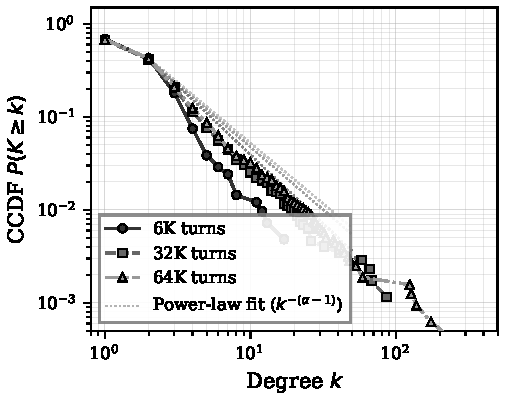
\includegraphics[width=0.85\columnwidth]{figures/fig_degree_distribution.pdf}
\caption{Complementary cumulative degree distribution (CCDF) on log-log axes. Dashed lines: MLE power-law fits. The heavy tail extends with scale.}
\label{fig:degree_dist}
\end{figure}

\subsection{Cross-task Contamination}

We additionally test whether propagation damage bleeds into unrelated tasks.
Using the Accurate\_Retrieval split from MemoryAgentBench, BFS propagation triggered during FactConsolidation degrades retrieval F1 by $10.1\pm1.6$pp across the top-5 hub entities.
\attraware{} preserves full accuracy (F1 $71.1\pm1.3$\% vs baseline $70.9$\%).
Full results are in \cref{app:cross_task}.
The severity of organic damage raises a natural question: can an adversary deliberately target hub entities to amplify this effect?


% ============================================================
\section{Hub-Targeted Amplification}
\label{sec:c3}

\subsection{Threat Model}

We evaluate three attacker knowledge levels: \textbf{black-box} (general knowledge), \textbf{gray-box} (hub entity names known), and \textbf{white-box} (fact registry access).
The attacker injects facts through the system's normal memory write interface; conflict detection triggers when a new fact maps to an existing subject-key, initiating the propagation cascade under study.

\subsection{Results}

\begin{table}[htbp]
\centering
\footnotesize
\begin{tabular}{lrrrr}
\toprule
\textbf{Attack} & \textbf{BFS Dam.} & \textbf{BFS Kill} & \textbf{Attr Dam.} \\
\midrule
\multicolumn{4}{l}{\textit{6K Context (344 valid memories)}} \\
1 fact & 5.2\% & 0.3\% & 0.0\% \\
3 facts & 26.7\% & 4.4\% & 0.0\% \\
5 facts & 39.8\% & 17.4\% & 0.3\% \\
\midrule
\multicolumn{4}{l}{\textit{32K Context (1,744 valid memories)}} \\
1 fact & 38.1\% & 1.0\% & 0.0\% \\
5 facts & \textbf{57.3\%} & \textbf{19.3\%} & 1.0\% \\
\bottomrule
\end{tabular}
\caption{White-box adversarial results. Kill = weight $< 0.1$.}
\label{tab:adversarial}
\end{table}

\finding{4} A single fake fact damages 5.2\% (6K) to 38.1\% (32K) of valid memories (\cref{tab:adversarial})---$7.3\times$ amplification from scale alone.
Five facts at 32K degrade 57.3\%, with 19.3\% killed (weight $< 0.1$).

\begin{table}[htbp]
\centering
\footnotesize
\begin{tabular}{lrrr}
\toprule
\textbf{Attack} & \textbf{Facts} & \textbf{Hit} & \textbf{BFS Dam.} \\
\midrule
White-box & 5 & 100\% & 39.8\% \\
Gray-box & 5 & 100\% & 20.9\% \\
Black-box & 5 & 0\% & 0.0\% \\
\bottomrule
\end{tabular}
\caption{Attack comparison at 6K. Black-box fails entirely; gray-box achieves 52\% of white-box damage.}
\label{tab:blackbox}
\end{table}

\finding{5} \Cref{tab:blackbox} shows that under our random-entity black-box baseline, attacks fail to hit hub entities (0\% hit rate).
More sophisticated strategies targeting high-frequency entities remain unexplored; our results establish that \textit{at minimum} gray-box knowledge of graph structure is needed for the attack vector studied here.

\begin{figure}[ht]
\centering
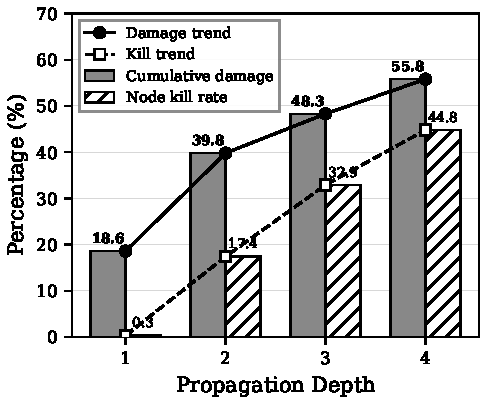
\includegraphics[width=0.85\columnwidth]{figures/fig_propagation_damage.pdf}
\caption{Propagation depth vs collateral damage (6K, 5-fact attack). Damage grows sublinearly while kill rate accelerates due to cumulative decay.}
\label{fig:depth}
\end{figure}


% ============================================================
\section{\attraware{} Selective Propagation}
\label{sec:c4}

\subsection{Method}

When fact $f$ with subject\_key \texttt{Entity:Attribute} is invalidated, \attraware{} restricts propagation to attribute-directed downstream dependencies (\cref{alg:attraware}):

\begin{algorithm}[htbp]
\caption{\attraware{} Selective Propagation}
\label{alg:attraware}
\begin{algorithmic}[1]
\REQUIRE Invalidated fact $f$ with key $s{:}a$, graph $G$, registry $R$, max depth $D$, decay $\delta$, current depth $h{=}0$
\STATE $s \leftarrow$ subject entity of $f$
\STATE $E_{\text{obj}} \leftarrow$ entities linked to $f$ in $G$, $e \neq s$
\FOR{each $e \in E_{\text{obj}}$}
  \STATE $M_{\text{down}} \leftarrow \{R[k] \mid k.\text{entity} = e\}$ \COMMENT{facts where $e$ is subject}
  \FOR{each $m \in M_{\text{down}}$ if $m$ is valid}
    \STATE $d_{\text{in}} \leftarrow \max(\text{in\_degree}(e, G), 1)$
    \STATE $m.w \leftarrow m.w \times (1 - \frac{1-\delta}{d_{\text{in}}})$
    \IF{$h < D$}
      \STATE \textbf{Propagate}($m, G, R, D, \delta, h{+}1$)
    \ENDIF
  \ENDFOR
\ENDFOR
\end{algorithmic}
\end{algorithm}

The key filtering step is line~4: instead of visiting all graph neighbors, \attraware{} retrieves only facts where the object entity appears as \textit{subject}---restricting propagation to downstream attribute-directed chains.
\attraware{} does not infer causality directly; it uses attribute-keyed directionality as a conservative proxy for dependency.
The in-degree adjustment (line~6) dampens decay for highly-connected entities.
\bfsprop{} differs by visiting all neighbors without semantic filtering or in-degree adjustment.
All operations are string-matching or arithmetic over pre-existing metadata---\textbf{no LLM calls} at propagation time; each step completes in $<$10\,ms.
The full \attraware{} pipeline processes 64K-scale graphs in $<$1\,s without GPU.

\subsection{Defense Comparison}

\begin{table}[htbp]
\centering
\footnotesize
\begin{tabular}{lrrrr}
\toprule
\textbf{Defense} & \textbf{Dam.} & \textbf{Kill} & \textbf{EM} & \textbf{F1} \\
\midrule
\bfsprop{} (no cap) & 39.8\% & 17.4\% & 10.0\% & 13.3\% \\
Degree-cap=5 & 24.1\% & 8.1\% & 10.0\% & 13.3\% \\
\attraware{} & \textbf{0.3\%} & \textbf{0.0\%} & \textbf{20.0\%} & \textbf{23.3\%} \\
\bottomrule
\end{tabular}
\caption{Defense comparison (6K, 5-fact attack). \attraware{} is $80\times$ more effective than the best structural defense.}
\label{tab:defense}
\end{table}

\finding{6} Degree capping reduces damage but remains $80\times$ worse than \attraware{}.
In our experiments, structural defenses did not substitute for semantic propagation filtering (\cref{tab:defense}).

\subsection{Cross-experiment Consistency}

\begin{table}[htbp]
\centering
\footnotesize
\begin{tabular}{lrrr}
\toprule
\textbf{Experiment} & \textbf{BFS} & \textbf{Attr} & \textbf{Def.} \\
\midrule
Scale 6K--64K & 69--79\% & 15\% & 78--81\% \\
Cross-task (F1) & $-$10.1pp & +0.0pp & 100\% \\
Adv 6K / 5f & 39.8\% & 0.3\% & 99.3\% \\
Adv 32K / 5f & 57.3\% & 1.0\% & 98.2\% \\
\bottomrule
\end{tabular}
\caption{\attraware{} defense effectiveness across all experiments. Cross-task: BFS propagation from hub entities degrades F1 by $10.1\pm1.6$pp on unrelated retrieval; \attraware{} preserves accuracy.}
\label{tab:defense_all}
\end{table}

\finding{7} \Cref{tab:defense_all} shows that \attraware{} achieves 78--100\% defense effectiveness across all experimental conditions---organic damage, adversarial attacks, and cross-task contamination.


% ============================================================
\section{Related Work}
\label{sec:related}

\paragraph{Memory invalidation and belief revision.}
Kumiho~\citep{kumiho_2026} maps AGM belief revision postulates~\citep{agm_1985} to a property graph with typed dependency edges, providing formal guarantees that unrelated beliefs are preserved.
Our work is complementary: Kumiho shows \textit{why} typed edges are needed (axiomatic); we show \textit{what happens without them} (empirical), providing the damage quantification that motivates architectural choices like Kumiho's.
MaRS~\citep{mars_2025} compares six forgetting policies with provenance closure constraints on the retention side; our study addresses the invalidation side.

\paragraph{Memory security.}
MINJA~\citep{minja_2025}, AgentPoison~\citep{agentpoison_2024}, and ER-MIA~\citep{ermia_2026} inject malicious content.
KEPo~\citep{kepo_2026} and LogicPoison~\citep{logicpoison_2026} manipulate graph topology.
Our attack is structurally distinct: it triggers the system's own forgetting mechanism rather than injecting content or manipulating retrieval paths.

\paragraph{Network resilience.}
Heavy-tailed networks exhibit robust-yet-fragile behavior under targeted hub removal~\citep{albert_attack_2000, cohen_percolation_2000}.
Our results empirically confirm this in AI memory graphs ($\alpha \approx 2.7$--$3.0$, heavy-tailed).


% ============================================================
\section{Discussion and Conclusion}
\label{sec:conclusion}

\paragraph{Key message.}
Our results identify \textbf{memory graph propagation} as a potential failure mode that creates an attack surface.
If graph-based propagation is adopted---a plausible evolution as memory scales demand consistency beyond individual facts---unfiltered co-occurrence traversal produces severe collateral damage (69--79\%), enables low-cost adversarial attacks (5 facts $\rightarrow$ 57.3\% degradation), and contaminates unrelated tasks (F1 $-$10.1pp).
\attraware{} provides practical defense (78--100\% effectiveness, no LLM calls during propagation) by enforcing attribute-directed filtering.

The principle is clear: \textbf{propagation must follow attribute-level dependency, not structural co-occurrence}.
This insight, well-established in transportation network resilience, is newly applied to AI memory systems.

\paragraph{Implications for memory system design.}
Systems adopting unfiltered propagation over untyped co-occurrence graphs may be vulnerable to hub-amplified damage unless propagation is dependency-constrained.
The attack is low-cost (5 facts), scales with memory size, and operates through legitimate maintenance pathways---making it harder to detect than content-injection attacks.
Hub entities (``United States'', ``Google'', a user's name) reflect genuine reality; removing them is not viable since they are essential for retrieval.
\attraware{} functions as a \textit{safety guardrail}, constraining \textit{any} propagation strategy---including learned policies such as RL-based retention scoring~\citep{mars_2025}---to plausible dependency chains.
\attraware{} is complementary to policy-learning approaches.

\paragraph{Generalizability.}
Entity mention frequencies in natural language follow Zipf's law~\citep{zipf_1949}: a small number of entities account for disproportionate mentions.
Co-occurrence graphs inherit this skew, producing hub-and-spoke structures regardless of domain---consistent with semantic network research~\citep{steyvers_semantic_2005, barabasi_scalefree_1999}.
While replication on additional benchmarks is important, the Zipfian origin of hub formation suggests our results generalize beyond MemoryAgentBench.

\paragraph{Limitations.}
(1) Single benchmark (MemoryAgentBench); the Zipfian argument above is theoretical, not empirical.
(2) Single LLM (Gemma-4-31B-it); while entity extraction is rule-based and graph topology drives core findings, LLM-dependent conflict detection may behave differently across model families---replication with diverse LLMs is an important next step.
(3) \attraware{}'s 15\% residual damage is not classified into legitimate cascade vs.\ false positive.
(4) Propagation parameters (depth=2, decay=0.5) are fixed; preliminary depth analysis (\cref{fig:depth}) shows damage grows sublinearly with depth, but systematic sensitivity sweeps across depth$\times$decay configurations remain for future work.
(5) Co-occurrence clique construction may amplify hub degrees compared to alternative graph topologies; our results should be interpreted as a stress-test setting.
(6) No current deployed memory system implements the BFS invalidation policy evaluated here; we evaluate a natural design extension that may arise as systems seek consistency beyond per-fact updates.

\paragraph{Future work.}
(1) Replace co-occurrence with typed-relation graphs and compare propagation behavior.
(2) Validate on production memory systems (Mem0$^g$, Zep) once they implement propagation.
(3) Although our experiments use text-derived fact graphs, the underlying issue is not text-specific: multimodal agents increasingly maintain episodic, semantic, and visual memories that share entity references, and the same co-occurrence-versus-dependency distinction arises when updates in one modality should or should not invalidate entries in another.

% ============================================================
\section*{LLM/Agent Usage Disclosure}

This research used LLM-based tools in three capacities:
(1)~Literature search and survey assistance (paper discovery and classification);
(2)~LaTeX editing and proofreading;
(3)~Experimental code development (benchmark integration, graph analysis scripts).
All experimental results, analysis, and conclusions were produced and validated by the authors.
The core experimental pipeline (entity extraction, subject-key matching, propagation algorithms) uses rule-based methods without LLM involvement at runtime, except for conflict detection which uses Gemma-4-31B-it as specified in the experimental setup.


% ============================================================
\bibliography{references}
\bibliographystyle{icml2026}


% ============================================================
\appendix

\section{Cross-task Contamination (C2)}
\label{app:cross_task}

BFS propagation from a single hub entity (``Debbie'', degree=715) cascades to 3,381 memories, causing EM $-5.0$pp and F1 $-18.2$pp on completely unrelated retrieval queries.
Across the top-5 hubs, BFS consistently degrades F1 by $10.1\pm1.6$pp.
\attraware{} preserves full accuracy (F1 $71.1\pm1.3$\% vs baseline $70.9$\%).

\section{Multi-run Statistics}
\label{app:stats}

We run the 6K adversarial attack 7 times (19 paired observations).
Pooled Wilcoxon signed-rank test: $W = 86.0$, $p = 0.0022$; bootstrap 95\% BCa CI $[2.82, 15.67]$pp excludes zero.
A mixed-effects model with attack strength as fixed effect and run as random intercept confirms the 5-fact condition is significant ($p = 0.020$).

\section{Graph Construction}
\label{app:graph}

Entity extraction uses rule-based proper noun detection and ``the X of Y'' patterns.
Co-occurrence edges form cliques per fact.
Subject-keys are deterministic: ``the president of Russia is Putin'' $\rightarrow$ \texttt{Russia:president}.
Conflict is triggered when a new fact maps to an existing subject-key.

\section{Experimental Configuration}
\label{app:config}

LLM: Gemma-4-31B-it (temp=0.0). Embedding: BAAI/bge-m3 (1024-dim). Graph: NetworkX DiGraph. Storage: SQLite in-memory. Benchmark: MemoryAgentBench (ICLR 2026). Scales: 6K/32K/64K. Propagation: depth=2, decay=0.5.


\end{document}
